%!TEX root = flock-comment-main.tex

\section*{Introduction}
Methods for the unsupervised clustering of genotypes have received 
considerable attention in the molecular ecology literature.  
The best known example of this class of methods is {\sc structure} 
\citep{Pritchardetal2000}, with over 12,000 citations identified on 
Google Scholar.  A variety of other 
clustering methods have been developed that are all closely related to 
{\sc structure}, for example {\sc NewHybrids} \citep{And&Tho2002}, {\sc 
BayesAss+} \citep{Wil&Ran2003}, and {\sc baps} 
\citep{Coranderetal2004}. An overview of the similarities between several of these methods can be 
found in \citet{Anderson2009PGAC}.

The recently introduced software {\sc flock} \citep{Duc&Tur2009} has
been described
as a ``non-Bayesian method [that] 
differs substantially from previous 
clustering algorithms'' \citep[][p.~1333]{Duc&Tur2009}. As reported
in a later paper, ``{\sc flock} is very different from  other clustering 
programs. It does not sample the space of partitions through small 
random step walks as in MCMC, and it does not try to optimize some 
target function, such as HWLE\@. Briefly stated, it is not based on a 
probabilistic search algorithm. On the contrary, {\sc flock} is 
entirely deterministic'' \citep[][p.~736]{Duc&Tur2012}.

However, here we identify 
the close relationship between {\sc flock}'s algorithm and the program
{\sc structure}.  Although the algorithm in {\sc flock}
is, as the authors point out, deterministic (apart from a random initial allocation of 
individuals to clusters), it can be interpreted as a 
limiting case of a probabilistic search algorithm applied to one of {\sc structure}'s
models.  More specifically, the {\sc flock} 
algorithm is a special case of the simulated annealing
algorithm for finding the Bayesian maximum-{\em a-posteriori}
estimate from a marginalized form of the {\sc structure} model with no
admixture and non-correlated allele frequencies.  

Being able to interpret {\sc flock} in this fashion should help users
interpret output from {\sc flock} and predict when it might and might not
give substantially different results than {\sc structure}. Below we describe
the correspondence between the programs in more detail, and then, for illustration, compare
the results obtained from {\sc flock} and {\sc structure} on a large, real data
set.

\section*{Comparison of methods}
We start with a succinct mathematical description of the {\sc structure}
model, then describe the {\sc flock} algorithm, and finally explain
the close relationship between the two.


\subsection*{{\sc structure}}
In the {\sc structure} model with no admixture (which, it should be pointed out, 
is not the default model in {\sc structure}), the unknown ``subpopulation'' that the 
$i\thh$ individual ($i=1,\ldots,N)$ belongs to is denoted by $Z_i \in \{1,\ldots,K\}$, 
where $K$ is the 
number of subpopulations (or clusters, as they are often referred to).  
In a diploid individual from cluster $k$, the 
allelic types of the two gene copies at the $\ell\thh$ locus are assumed
to be drawn independently from the vector of allele frequencies at
locus $\ell$ in subpopulation $k$,  $\theta_{k\ell}=(\theta_{k\ell 1},\ldots,\theta_{k\ell A_\ell})$, where 
$A_\ell$ 
denotes the number of alleles observed in the data set at locus $\ell$.
Hence, if $Y_{i\ell}$ denotes a vector of length $A_\ell$ whose components denote the 
number
of copies of each of the $A_\ell$ alleles at locus $\ell$ in a diploid individual $i$, and 
$Z_i=k$, then $Y_{i\ell}$ follows the multinomial distribution of two trials with
$A_\ell$  components and cell probabilities given by the allele frequencies: 
\begin{equation}
(Y_{i\ell}~|~Z_i=k) \sim \mathrm{Mult}_{A_\ell}(2, \theta_{k\ell}).
\end{equation}
In the {\sc structure} model without physical linkage, the genotypes at the loci are assumed to
be independent of one another, so the probability of the genotype data at
all $L$ loci---$Y_i=(Y_{i1},\ldots,Y_{iL})$---is simply a product of multinomial 
probabilities.
In the uncorrelated allele frequencies model, the prior on each $\theta_{k\ell}$ is a
Dirichlet distribution with parameters $(\lambda_{k\ell1},\ldots,\lambda_{k\ell A_
\ell})$,
which are usually all set to a value such as 1 or $1/A_\ell$.  

After initializing the unknown allele frequencies, $\theta = (\theta_1,\ldots,\theta_K)$, to randomly drawn values,
$\theta^{(0)}$, inference in the model proceeds by sampling from the joint posterior of the 
$Z_i$'s and $\theta$ using Gibbs sampling.  That is,
at iteration $t = 0, 1, 2, \ldots$:
\begin{enumerate}
\item each $Z^{(t)}_i$ is updated to $Z^{(t+1)}_i$ by sampling a value from 
the full conditional distribution of $Z_i$ given
$Y_i$ and $\theta^{(t)}$ (the current estimate of the allele frequencies).  This
distribution is found using Bayes' theorem. In {\sc structure}'s formulation, the 
prior probability that $Z_i=k$ is $1/K$ for all $k=1,\ldots, K$.     
\item $\theta^{(t)}$ is updated to $\theta^{(t+1)}$ from its full conditional distribution.  For each 
cluster
$k$ and locus $\ell$, the full conditional for $\theta_{k\ell}$ is independently a 
Dirichlet distribution with parameters $\lambda_{k\ell j} + \#(k,\ell,j)$, for 
$j=1,\ldots, A_\ell$,
where $\#(k,\ell,j)$ is the number of alleles of type $j$ at locus $\ell$ observed in 
individuals with $Z^{(t+1)}_i = k$.   
\end{enumerate}

It will be useful for our comparison with {\sc flock} to point out that another way 
of pursuing inference in this model would be to first integrate out the 
Dirichlet priors on the allele frequencies and then sample from the posterior
for the $Z_i$'s by Gibbs sampling.  When $\theta$ is integrated out, the genotypes 
of the individuals are no longer conditionally independent (they were originally
independent {\em conditional} on $\theta$ and the $Z_i$'s), so the calculation of 
the full conditional distribution of $Z_i$ becomes somewhat more involved,
but can be computed by the following reasoning. First, the 
conditional distribution of $Y_{i\ell}$, given that individual $i$ is from subpopulation $k$
(\ie $Z_i=k$), depends on the 
cluster memberships and genotypes at locus $\ell$ of all the remaining individuals,
which we denote by  $Z_{(-i)}$ and $Y_{(-i)\ell}$, respectively.
This full conditional for $Y_{i\ell}$ follows 
a Compound Dirichlet Multinomial distribution (CDM):
\begin{eqnarray}
\lefteqn{(Y_{i\ell}~|~Z_i=k,~Z_{(-i)},~Y_{(-i)\ell}) \sim} \label{eq:cdm}\\
& & \mathrm{CDM}(\lambda_{k\ell 1} + \#_{(-i)}(k,\ell,1), \ldots,
\lambda_{k\ell A_\ell} + \#_{(-i)}(k,\ell,A_\ell)), \nonumber
\end{eqnarray}
where $\#_{(-i)}(k,\ell,j)$ is the number of alleles of type $j$ at locus $\ell$
found in individuals {\em other than individual $i$} that currently
belong to cluster $k$. Thus, calculating the product of (\ref{eq:cdm}) across all the loci
($\ell = 1,\ldots,L$) gives the full conditional multilocus genotype probability 
for individual $i$:
\begin{eqnarray}
\lefteqn{P(Y_{i}~|~Z_i=k,~Z_{(-i)},~Y_{(-i)}) =}  \label{eq:cdm-multi-prob} \\
& &  \prod_{\ell=1}^L P(Y_{i\ell}~|~Z_i=k,~Z_{(-i)},~Y_{(-i)\ell}). \nonumber
\end{eqnarray}
Computing (\ref{eq:cdm-multi-prob}) for 
for each value of $Z_i=k \in 
\{1,\ldots,K\}$ 
and normalizing to sum to one gives the full conditional distribution for 
$Z_i$:
\begin{equation}
P(Z_i=k~|~Y_i, ~Z_{(-i)},~Y_{(-i)})~~,~~k=1,\ldots,K.
\label{eq:fc}
\end{equation}
A new value of $Z_i$ would be drawn from (\ref{eq:fc}) if doing Gibbs sampling in this
version of the {\sc structure} model in which $\theta$ has been integrated out.  In 
fact,
this is the approach (with a slightly different prior weight on the $Z_i$'s) taken to 
update 
$Z_i$ in both {\sc hwler} \citep{Pel&Mas2006} and {\sc structurama} \citep{Hue&And2007} 
when not
proposing changes to the number of clusters.



\subsection*{{\sc flock}}
Here we translate the procedure given by \citet{Duc&Tur2009} for the 
{\sc flock} algorithm into a specification in terms of the variables
defined in the previous section.  We provide the description for a case in which
it is assumed there are $K$ clusters.

The first step of the flock algorithm is initialization, during which 
the program randomly allocates each of the $N$ individuals to one of 
$K$ clusters.  Then a number of reallocation steps are performed.  During every one of 
these steps, each individual is given the chance to be reallocated 
(\ie moved to a different cluster).  This is done on the basis of 
maximum likelihood: as \citeauthor{Duc&Tur2009} say (2009, p.~1335), ``Re-allocations are 
performed following multilocus maximum likelihood (Paetkau et al. 1995).''

From that description, it is not clear how \citeauthor{Duc&Tur2009} treat 
alleles that appear in the focal
individual but do not appear within any other individuals within a cluster.
The original approach of \citet{Paetkauetal1995} merely added 0.01 or some other
small value to each allele frequency that was 0, and then renormalized 
the allele frequencies to sum to 1.  In later works, Paetkau and colleagues
also employed the ``Bayesian'' approach of \citet{Ran&Mou1997} in their 
software {\sc geneclass2}  \citep{Piryetal2004}.  If \citeauthor{Duc&Tur2009}
use the approach of \citet{Ran&Mou1997}, then the $i\thh$ individual will
be reallocated to whichever cluster gives the highest value to 
$P(Y_{i}~|~Z_i=k,~Z_{(-i)},~Y_{(-i)})$, which is 
exactly the probability
defined in (\ref{eq:cdm-multi-prob}).  
If \citeauthor{Duc&Tur2009} use the simpler ``add 0.01 and renormalize''
formulation of \citet{Paetkauetal1995}, then their reallocations are based
on maximizing a likelihood that, although it may not be formally identical to
the probability defined in (\ref{eq:cdm-multi-prob}), is nearly identical to it.   

It is worth pointing out that, since the
{\sc structure} model without admixture assumes a uniform prior over 
the $K$ different clusters, $P(Y_{i}~|~Z_i=k,~Z_{(-i)},~Y_{(-i)})$
is exactly proportional to $P(Z_i=k~|~Y_i, ~Z_{(-i)},~Y_{(-i)})$, which 
we have shown is the
full conditional distribution for $Z_i$ in the {\sc structure} model after
integrating out $\theta$.  Thus, we have shown that, doing Gibbs
sampling for $Z_i$ in  the {\sc structure} model in which $\theta$ has been
integrated out would involve sampling a new value of $Z_i$ from the 
probability distribution,
\[
P(Z_i=k~|~Y_i, ~Z_{(-i)},~Y_{(-i)})
\]
and that the updates that
{\sc flock} makes to each $Z_i$ involve assigning to $Z_i$
\begin{equation}
\arg\max_k P(Z_i=k~|~Y_i, ~Z_{(-i)},~Y_{(-i)}),
\end{equation}
\ie the value of $k$ that maximizes $P(Z_i=k~|~Y_i, ~Z_{(-i)},~Y_{(-i)})$
(or, as stated above, a nearly identical function of $k$, depending on how
the program {\sc flock} treats alleles that are not observed in certain clusters).



\subsection*{The {\sc flock} algorithm and {\sc structure}}
The goal of {\sc structure}'s MCMC algorithm is to sample from the space of 
$Z$'s in proportion to their posterior probability.  If, all that was desired
was a point estimate of the $Z_i$'s that maximized the posterior probability,
then one standard approach to finding that maximum-{\em a-posteriori}, or MAP, 
estimate, would be to use simulated annealing \citep{Kirkpatricketal1983}.
To do simulated annealing in the {\sc structure} model with no admixture and
no correlated allele frequency prior, after integrating out the unknown
allele frequencies, the updates for each $Z_i$ would be made from the 
distribution
\[
\biggl[P(Z_i=k~|~Y_i, ~Z_{(-i)},~Y_{(-i)})\biggr]^\beta
\]
which is the same full conditional distribution as the marginalized {\sc structure}
model (equation~\ref{eq:fc}), raised
to the power $\beta$.  In typical applications of simulated annealing,
$\beta$ is set to a starting value less than 1, and, as the algorithm proceeds,
$\beta$ is increased according to a ``cooling schedule''\citep{Hajek1988}, until
the algorithm finds a local maximum in the posterior probability surface.  
When $\beta$ is small, the process can easily traverse ``valleys''
in the posterior probability surface and has a better chance of searching
more of the space for the maximum value.  As $\beta$ gets larger, it becomes
more probable that the process will
move uphill on the probability surface, tending toward the local
maximum near where it currently is.    

It should now be clear that the algorithm in {\sc flock} is a simulated annealing 
algorithm for the {\sc structure} model in which the cooling schedule is
``start with $\beta\rightarrow\infty$ and leave it there for the duration of 
the algorithm.''  As such, we can expect that it may be more susceptible 
to becoming trapped in local modes of the posterior probability. 
In the following section we show that {\sc structure} and {\sc flock} find similar
solutions in the analysis of a large microsatellite data set, though, as expected,
{\sc flock} seems to find the same solution less consistently than does {\sc structure}.



\section*{Comparison of {\sc structure} and {\sc flock} results}
Data sets with known $K$ were simulated
(code provided on GitHub repository https://github.com/eriqande/flock-comment)
and evaluated in the programs {\sc flock} and {\sc structure} 
for the known value.The first dataset simulated was composed of five populations of 
sizes 500, 500, 800, 1100, and 1100 comprised of individuals 
with 15 loci and an average pairwise $F_{ST} = 0.03$ between populations. 
The second and third dataset were simulated with population sizes
250, 250, 400, 550, and 550 and average pairwise $F_{ST} = 0.02 and 0.01$
respectively. {\sc flock} was run nine times using the default setting for all 
run parameters (initial partition = random, number of iterations = 20, number of runs = 50, 
LLOD threshold = 0) for the known value of $K$. The no-admixture, 
uncorrelated-allele-frequency model implemented in {\sc structure} was run nine times with 
a 5,000 sweep burn-in followed by a 20,000 sweep sample from the posterior. 
% Looking back some of the runs were under different conditions, not huge differences. 
% But 1000 burn-in and 5,000 sweep look about the same
All runs were performed on a JNCS D685 with an i7 3.40GHz processor and 8GB
of RAM running 64-bit Windows 7. 

For each set of runs, {\sc flock} reports the 
normalized likelihood values (the exponentiated log-likelihood value for an individual's 
membership to each of $K$ clusters, scaled to sum to one) for a run belonging to the 
longest plateau - refered to as the 'best run' by \citep{Duc&Tur2012} (see below).
These values can be compared to the $q_i$ values
returned by {\sc structure}, which, in the no-admixture case, are posterior probabilities of cluster membership.
The program {\sc clumpp} \citep{Jak&Ros2007} was used to relabel clusters among different runs,
while the program {\sc district} \citep{Rosenberg2004} was used to plot individual \textit{$q_i$} values.

\citet{Duc&Tur2012} describe a method for using {\sc flock} to estimate, $K$, the number of
subpopulations. The user must specify both the number of runs (different initial allocations of individuals 
to each cluster) as well as the number of iterations. (In each iteration every individual has the opportunity to be reallocated 
to a different cluster.) At the conclusion of each run, the log-likelihood value for membership to all $K$ clusters is computed
and the log likelihood difference (LLOD), the difference between the cluster with the highest likelihood 
and second highest likelihood, is calculated for each individual. {\sc flock} identifies runs that 
have converged to the same solution by detecting that they have the same mean LLOD score, and, in 
{\sc flock} parlance, a series of runs that have converged to the same solution are termed a ``plateau.'' 
The plateau record is a list of how many runs converged to the same allocation
of individuals. 
\citet{Duc&Tur2012} developed two stopping rules that they use to estimate $K$.\citet{Duc&Tur2012} advocate running  {\sc flock} until either a single plateau of
$\geq 6$ runs is reached or four consecutive $K$ values yield no plateaus. If the first stopping condition is satisfied,
the $K$ for which there is a single plateau of $\geq 6$ runs is the point estimate for $K$. Alternatively, 
if multiple plateaus are observed with at least one plateau of $\geq 6$ runs, the largest value of $K$ that satisfies 
this conditon should be taken as the lower bound estimate of $K$. If no plateaus of $\geq 6$ runs are observed, $K$
is declared {\em undecided}.  
 
It is now common practice to use the approximate marginal likelihood ($\ln P(D)$) from {\sc structure}
or a derived quantity such as $\Delta K$ \citep{Evannoetal2005} to try to estimate $K$.
While we take the stance that estimates of $K$ made with {\em any} unsupervised clustering algorithm
from data on real (non-idealized) populations should always be interpreted and used
cautiously, it is nonetheless instructive to compare \citet{Duc&Tur2012}'s method for
estimating $K$ to results obtained using $\ln P(D)$ and $\Delta K$, and we do so, below. 

\subsection*{Results} 
Run times for both programs were relatively short, albeit in the case of {\sc flock} 
non-trivial. {\sc flock} averaged 67.3 minutes
for each run of the first simulated dataset, while each group of 
9 iterations for {\sc structure} averaged 18 minutes. CALCULATE
TIME FOR OTHER SIMULATIONS
 
{\sc flock} and {\sc structure} provide nearly identical results in 
terms of how individuals are allocated among runs for 
all simulations (Fig.~\ref{fig:Sims}). As $F_{ST}$ decreases 
between populations the solutions that {\sc flock} are more variable. 
The average Euclidean distance between the known $q_i$ value and 
the infered value from each program increases as the genetic 
differentiation among populations decreases. {\sc flock} had an 
smaller mean Euclidean distance over all runs for simulations 
1 and 2, but had much larger variation in simulation 3 (Fig.~\ref{fig:ED}).
%calculate Euclidean distance between flock and structure values. 
 
There was very little variation in the 'best-run' returned by {\sc flock}. 
From the nine different sets of runs for the first simulated dataset, 
three groups of runs ended with 
identical clusters (runs 2,8 \& 9, runs 1 \& 3, and runs 4 \& 7). 
Of the other 31 pairwise comparisions that were not identical
15 differed by the placement of 1 indvidual, 11 differed by the placement
of 2 individuals, and 5 differed by the placement of 3 individuals. 

Despite the similar allocation of individuals into $K$ clusters, the 
plateau analysis to estimate $K$ in {\sc flock} did not support $K = 5$. 
For the first simulated dataset plateaus of varioius lengths were observed, 
but none greater than 5 while no plateaus were observed for either second or 
third simulated datasets.

\begin{figure*}
\begin{center}
    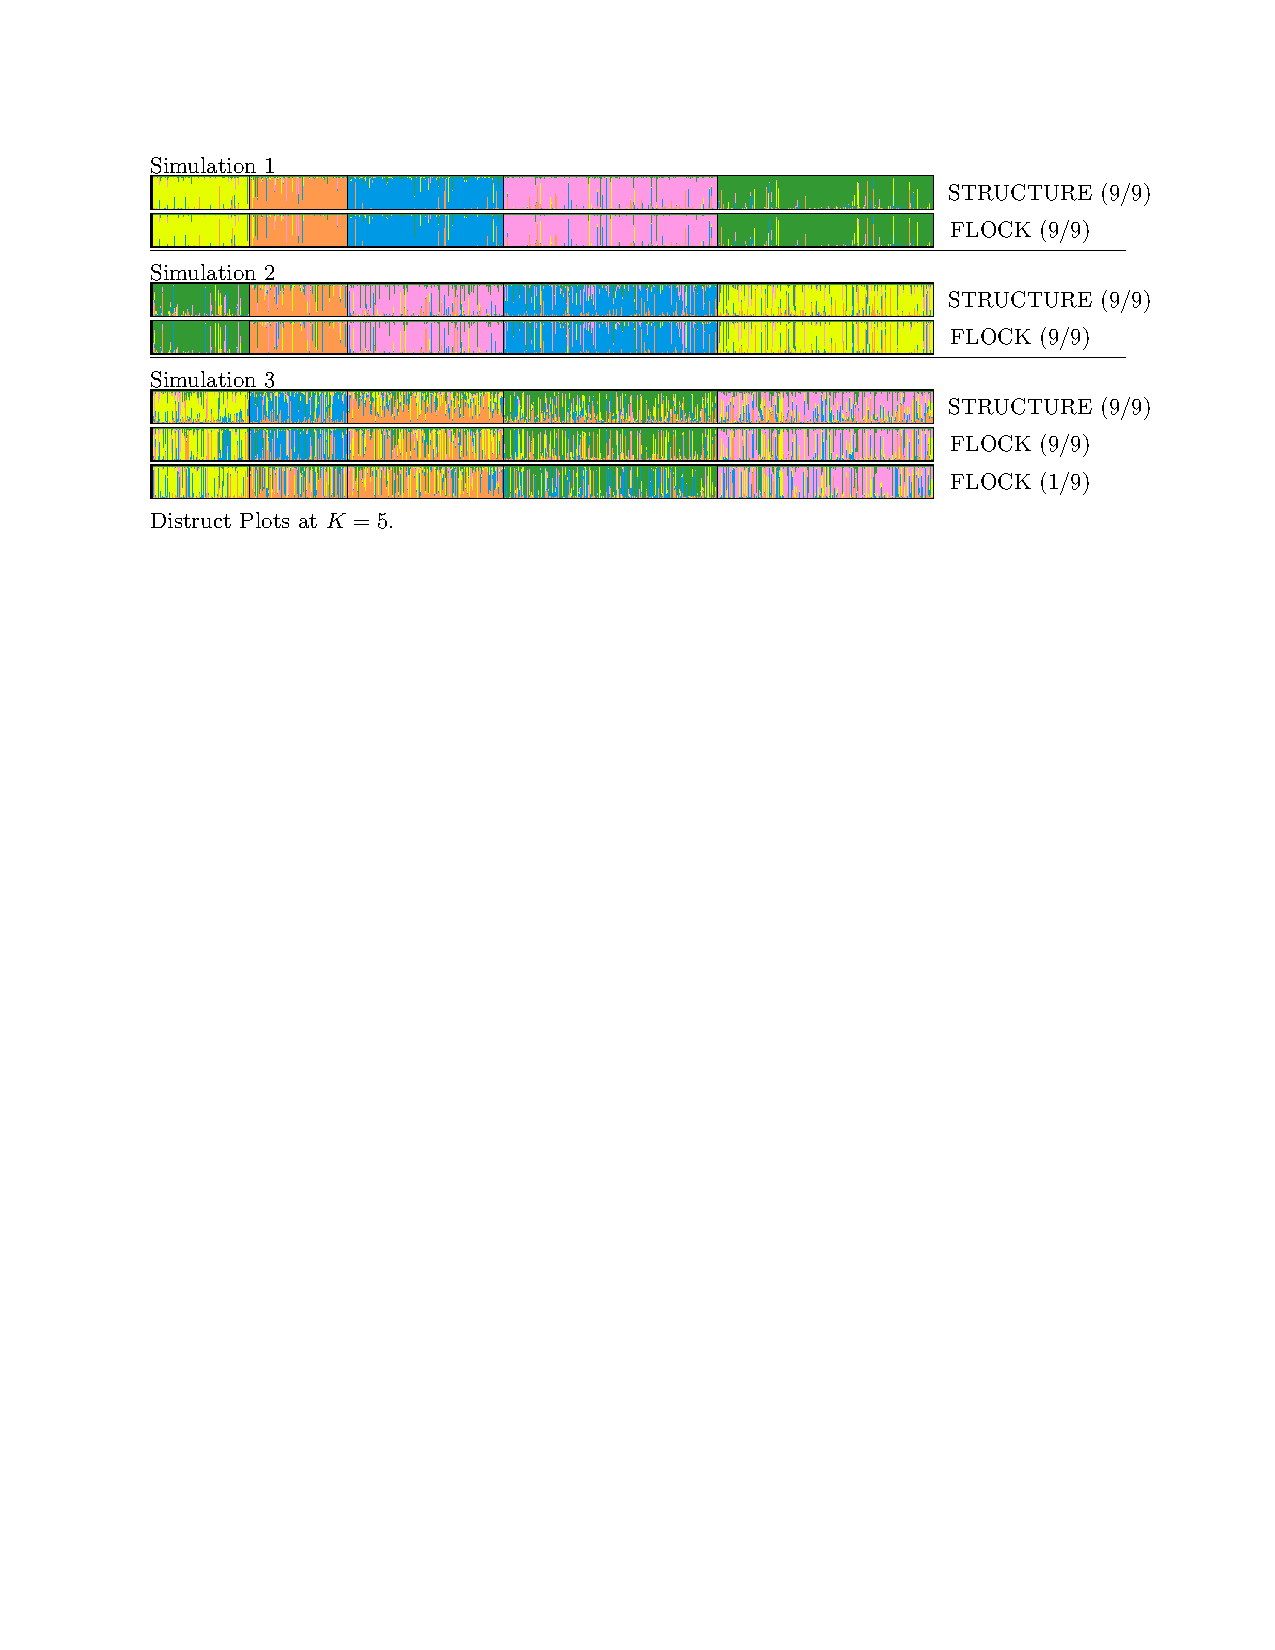
\includegraphics[width=\textwidth]{images/Figures-Pat/Simulations_Fig1.pdf}   % Use this if we want it color (I'll make greyscale later)  
    \caption{Plots of $q_i$ values from {\sc structure} and the normalized likelihood values 
of {\sc flock} made with the program {\sc distruct}. Each horizontal plot represents one of nine individual runs of the program {\sc structure}, or the `best run' from a series of nine runs in {\sc flock} at $K=5$. Within each plot 
$q_i$ values from {\sc structure} and the normalized likelihood values 
from {\sc flock}  are represented by a 
%gray-scale
vertical bar. Simulation 1 was composed of populations of 
size 500, 500, 800, 1100, and 1100 with an average pairwise $F_{ST} = 0.03$ between populations. 
The second and third dataset were simulated with population sizes
250, 250, 400, 550, and 550 and average pairwise $F_{ST} =$ 0.02 and 0.01
respectively.}
    \label{fig:Sims}
\end{center}
\end{figure*}

\begin{figure*}
\begin{center}
    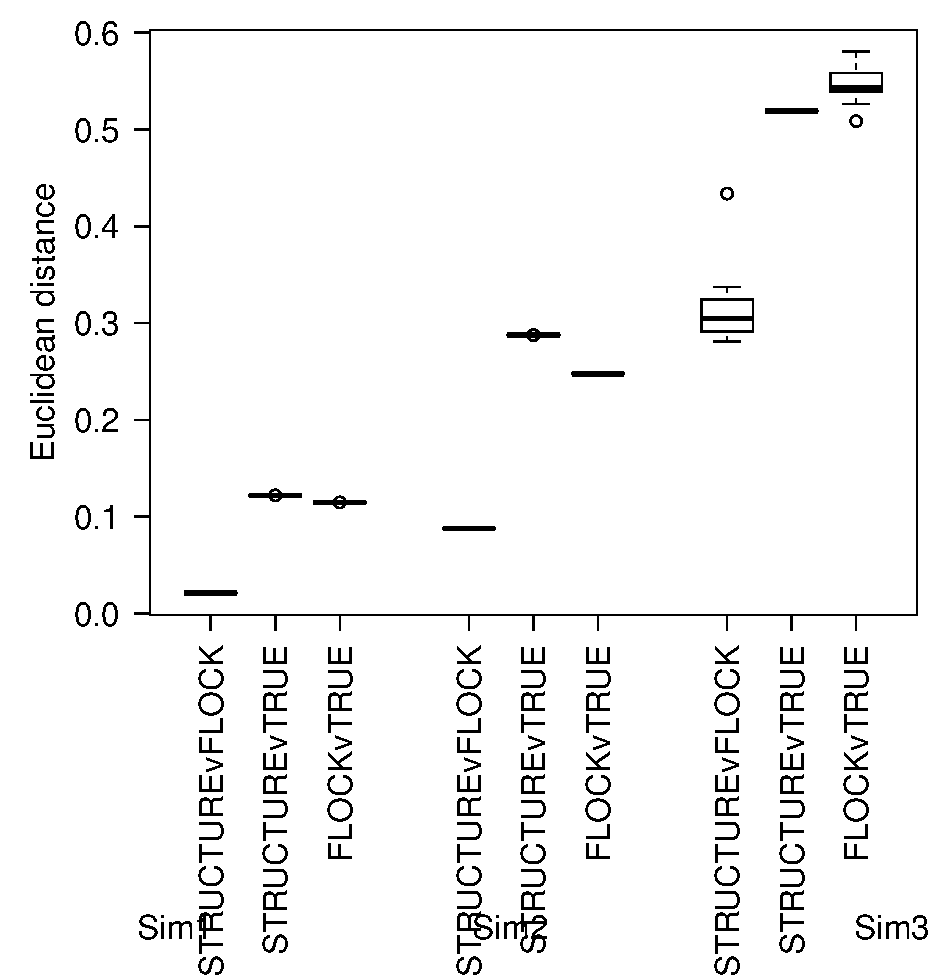
\includegraphics[width=0.5\textwidth]{images/Figures-Pat/ED_fig2.pdf}   
% HIDEOUS GRAPH, we will talk and I might make one with actual distributions! 
    \caption{Eucledian distance between true $q_i$ value and inferred value from {\sc structure} and {\sc flock} .}
    \label{fig:ED}
\end{center}
\end{figure*}

\section*{Conclusions}
In the past decade, the use of genetic markers to identify population structure and to attempt inference of
the number of genetic clusters ($K$) in a collection has dramatically increased in the fields of ecology, evolution, 
epidemiology, and conservation
genetics. The most commonly used program for doing this is {\sc structure} \citep{Pritchardetal2000,Falushetal2003}, 
a full-featured program with many options that is widely-used, well-tested, and universally regarded as a standard tool amongst molecular ecologists. 
We've shown here that the model incorporated by {\sc flock} is essentially equivalent to the no-admixture model with non-correlated allele frequencies within the program {\sc structure}. In comparing results from {\sc flock} and {\sc structure} 
on simulated datasets with varying levels of differnetiation among populations
we find that the two programs give similar results.

Though we observed similar results
between the two programs at low values of $K$, {\sc flock}'s `best-run' solutions became somewhat inconsistent at higher values of $K$.
This observation was consistent with \citet{Duc&Tur2012}'s comparison of the 
two programs using simulated data 
for $K=4$ \& 8, $L=10$ (Fig. 4 in \citet{Duc&Tur2012}). 
This is likely a consequence of the rapidly increasing size of the search space over possible 
partitions as $K$ and $n$, the number of individuals, increase. 
The likelihood surface defined on partitions of this space will often
be multimodal---possessing numerous local peaks and troughs.
The peak that  {\sc flock}'s algorithm finds is entirely determined by the initial, random, allocation of 
individuals, as the algorithm proceeds deterministically after the initial random allocation.
If the number of initial allocations does not increase
as $K$ is increased, the starting allocations become diffusely scattered in the space of all
possible partitions making it less likely that many (if any at all) will converge to the same local mode. 
This coupled with the fact that there is 
ambiguity in what defines a `best run' when all plateaus are of length zero complicates the interpretation
of results from {\sc flock} if no non-zero plateaus are encountered. The problem of getting 
caught in local modes is not unique to {\sc flock}---{\sc structure} also can converge to 
different solutions in complex spaces; however our results suggest this is a bigger problem for {\sc flock}.
By increasing the number of loci used in their simulations, \citet{Duc&Tur2012} showed  that 
{\sc flock} was able to converge in a simulated data set with $K=8$, but held no advantage in inference of $K$ over {\sc structure}. That simulated data set, with $n=240$ was considerably smaller and less complex than the real data investigated here.
%They simulated data using 500 individuals per population but only used 30 of them in the analysis.
% if you have more loci than individuals per population with high Fst between groups it does great!    

 
One of the advantages of {\sc flock} over other methods for genetic clustering
is reported to be the short processing time for each run of {\sc flock}.
While \citet{Duc&Tur2012} observed faster processing times (relative to other methods) in their 
comparisons, we did not observe this advantage in our analysis. This appears to result from two issues. First,
our example data set was an order of magnitude larger than the largest data set analyzed in \citet{Duc&Tur2012}.  
Second, in the comparison by \citet{Duc&Tur2012}, 
{\sc flock} was set to perform 50 runs and 20 iterations for each $K$ starting at 2 and ending when 
one of the stopping conditions was met, and computing times for that analysis were compared to ten iterations of 
the admixture and correlated allele frequency model in {\sc structure} using 
a 50,000 sweep burn-in followed 
by a 200,000 sweep sample from the posterior for values of $K$ from 1 to three more than the true 
value of $K$. 
To us it seemed reasonable to compare, for each $K$, the running times of one iteration of {\sc structure} (50,000 
burn in and 200,000 sample collection sweeps)
to one iteration of {\sc flock} (50 different starting allocations that are reallocated 20 times) 
as both were used to provide one of 6 total estimates (per value of $K$) of the partition of individuals into 
clusters. Though
it is difficult to reliably assess differences in program run times when there is no clear consensus on what 
constitutes a reasonable comparison with respect to run length and number of runs, our results indicate that {\sc flock} did not carry a distinct run-time advantage over {\sc structure}.

While there has been lengthy 
discourse over the choice of estimators for $K$ in {\sc structure} 
\citep{Pritchardetal2000,Evannoetal2005,Wap&Gag2006,Gaoetal2011}, less has been written on how the number of 
individuals
and the number of starting allocations can affect not only the convergence of different runs of {\sc flock}, but also its 
inference of $K$. \citeauthor{Duc&Tur2012} developed estimation rules for $K$ based on simulated data 
sets with a modest number of individuals and different migration regimes and rates, numbers of loci, and $K$. 
By relying on the number of identical partitions (mean LLOD values) obtained by {\sc flock} over multiple
runs as a means of supporting 
a particular $K$,  similar---but not identical---partitions
will provide no support to a given $K$. Given {\sc flock}'s tendency to converge to 
different solutions with large $K$ and $n$, it seems that 
this method for estimating $K$ is unlikely to be reliable or workable in large, complex
problems.  One possible patch for this problem would be running
multiple small batches and using the programs {\sc clumpp} \citep{Jak&Ros2007} and
{\sc distruct} \citep{Rosenberg2004} to visually inspect the `best run' results, and then 
determine plateaus amongst {\sc flock}'s replicate solutions not by identical LLOD, but by visual inspection of 
partitions that
are very similar but are perhaps not identical; however such an approach would be labor-intensive
and would rely on arbitrary, difficult-to-reproduce decisions.  It is probably better to use {\sc structure} in such cases, keeping in mind, of course, that
estimating $K$ is a hard problem and should only be undertaken with caution, regardless of the method 
used. This is especially true in real populations which do not conform to the assumptions of genetic clustering models.


We made our comparison between {\sc flock} and the {\em no-admixture} model in 
{\sc structure} which is not the default model used in {\sc structure}. Rather, by default, {\sc structure} uses 
its {\em with-admixture} model.  Such a model explicitly tries to account for the admixed origin
of individuals in the sample and thus may be a more appropriate model than the no-admixture model,
or {\sc flock}, when the sample contains individuals that are admixed between populations.  A further advantage
of the with-admixture model is that it allows inference of the population of origin of individual alleles at 
different loci within individuals, and not just of the individuals themselves.   We also note that {\sc flock} 
corresponds to {\sc structure}'s model with uncorrelated allele frequency priors. \citet{Falushetal2003} found that
using their ``$F$-model,'' which assumes that allele frequencies between populations are correlated {\em a priori}, 
allowed {\sc structure} to dissect more subtle population structure than was possible using the prior with
uncorrelated allele frequencies.  Modifying {\sc flock} so as to reap similar benefits from using a prior
with correlated allele frequencies seems like it would be an interesting challenge, though difficult
because {\sc flock}'s formulation effectively integrates the allele frequencies out of the model.
 


Often, newly-developed algorithms come to be understood within more general contexts and 
frameworks, and this, in turn, can help guide improvement of those algorithms.  For example, in population
genetics, the ``Markov recursion'' algorithm of \citet{Gri&Tav1994-AI} was identified by \citet{Felsensteinetal1999} 
as a special case of importance sampling \citep{Ham&Han1964}, a perspective which allowed 
\citet{Ste&Don2000} to improve upon the algorithm dramatically.  Here we have identified the {\sc flock}
algorithm as a limiting case of simulating annealing upon {\sc structure}'s no-admixture model with uncorrelated
allele frequencies. We hope this will
help users to understand and interpret {\sc flock}'s behavior and will provide insights that may be useful 
in the potential development of {\sc flock} or other clustering algorithms.   


\section*{Acknowledgments}
We are grateful to Kristen Ruegg and Robin Waples for helpful comments on a draft of this paper.